\documentclass[crop,class=article]{standalone}
%----------------------------Preamble-------------------------------%
\usepackage{amssymb}                % For \minus command.
\DeclareMathSymbol{\minus}{\mathbin}{AMSa}{"39} % Unary minus sign.
\usepackage{tikz}                   % Drawing/graphing tools.
\usetikzlibrary{
    angles,                 % Drawing angles within triangles.
    arrows.meta,            % Latex and Stealth arrows.
    quotes                  % Adding labels to angles.
}
%--------------------------Main Document----------------------------%
\begin{document}
    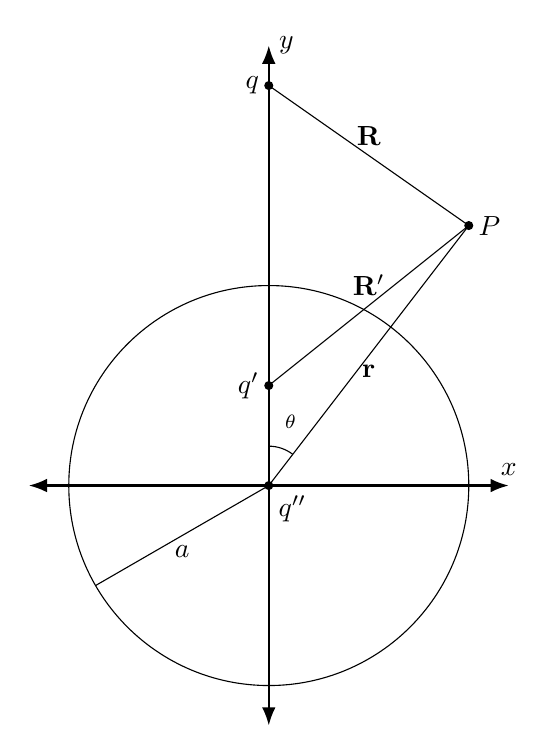
\begin{tikzpicture}[>=Latex]
        \coordinate (P) at (1in, 1.3in);
        \coordinate (q) at (0, 2in);
        \coordinate (q1) at (0, 0.5in);
        \coordinate (O) at (0,0);
        \draw[<->, thick] (-1.2in, 0) to (1.2in, 0)
            node [above] {$x$};
        \draw[<->, thick] (0, -1.2in) to (0, 2.2in)
            node [right] {$y$};
        \draw (0,0) circle (1in);
        \draw[fill, black] (O) circle (0.05cm)
            node [below right] {$q''$};
        \draw[fill, black] (P) circle (0.05cm) node [right] {$P$};
        \draw[fill, black] (q) circle (0.05cm) node [left] {$q$};
        \draw[fill, black] (q1) circle (0.05cm) node [left] {$q'$};
        \draw (O) to node [below] {$\mathbf{r}$} (P);
        \draw (P) to node [above] {$\mathbf{R}$} (q);
        \draw (q1) to node[above] {$\mathbf{R}'$} (P);
        \draw (O) to node [below] {$a$} (-0.866in, -0.5in);

        \pic[%
            draw=black,
            "\scriptsize{${\theta}$}",
            angle eccentricity=1.7,
            angle radius =0.5cm
        ]   {angle = P--O--q};
    \end{tikzpicture}
\end{document}